\documentclass{beamer}
% \usepackage[utf8]{inputenc}

\usepackage{amsmath, amsfonts, amssymb}
\usepackage{amsthm}
\usepackage{mathtools}
\usepackage{physics}
\usepackage[super]{nth}

\usepackage{graphicx}
\graphicspath{{../figures/}}

\usepackage{pgfplots}
\usepackage{tikz}
\usepackage{standalone}
\usepackage{subcaption}
\usepackage{siunitx}

\usepackage[english]{isodate}

% \usepackage{xcolor}
% \textcolor variant for math mode: \mathcolor
\makeatletter
\def\mathcolor#1#{\@mathcolor{#1}}
\def\@mathcolor#1#2#3{%
  \protect\leavevmode
  \begingroup
    \color#1{#2}#3%
  \endgroup
}
\makeatother

\newcommand{\ee}{\operatorname{e}}          % Euler's number
\newcommand{\ii}{\mathrm{i}}                % imaginary unit
\newcommand{\ad}[1]{a_{#1}^{\dagger}}       % creation operator
\newcommand*\mean[1]{\overline{#1}}         % mean

\usetheme[progressbar=frametitle]{metropolis}           % Use metropolis theme
% \usepackage{appendixnumberbeamer}
\setbeamercolor{background canvas}{bg=white}
% \usefonttheme{xefira}

\title{LASER WAKEFIELD ACCELERATION:\@ Studies using Particle in Cell Method}
\subtitle{Master Thesis}
\date{Bucharest, \today}
\author{Sebastian MICLUȚA-CÂMPEANU\\
Scientific Advisers\\
Prof.~dr.~Virgil BĂRAN \\
Conf.~dr.~Alexandru NICOLIN}

\institute{University of Bucharest}

\begin{document}
\maketitle%

%%%%%%%%%%%%%%%%%%%%%%%%%%%% slide 1 %%%%%%%%%%%%%%%%%%%%%%%%%%%%

\begin{frame}{Outline}
  \tableofcontents[]
\end{frame}

\section{Introduction}

%%%%%%%%%%%%%%%%%%%%%%%%%%%% slide 3 %%%%%%%%%%%%%%%%%%%%%%%%%%%%

\begin{frame}
  \begin{itemize}
	\item The aim of this thesis is to investigate the interaction of high power
	laser pulses with solid and gaseous targets.
    \item The fundamentals of the Particle in Cell method are detailed.
	\item A method of accelerating electrons with very intense lasers is presented.
  \end{itemize}
\end{frame}

\section{Classical Electrodynamics}

\begin{frame}{Maxwell's Equations}
	\begin{itemize}
		\item The dynamics of the electromagnetic fields are given by Maxwell's Equations
		\begin{subequations}%
		  \begin{align*}
		    \div{\vb{E}}  = \frac{\rho}{\varepsilon_0} &&
		    \div{\vb{B}}  = 0  \\
		    \curl{\vb{E}}  = - \pdv{\vb{B}}{t} &&
		    \curl{\vb{B}}  = \mu_0 \vb{j} + \frac{1}{c^2} \pdv{\vb{E}}{t}
		  \end{align*}
		\end{subequations}
		\item The dynamics of the charged particles are given by
		\begin{align*}
		  \dv{\vb{x}}{t} &= \vb{v} \\
		  \dv{\vb{v}}{t} &= \frac{q}{m} \left(\vb{E} + \vb{v}\cp\vb{B}\right)\,.
		\end{align*}
	\end{itemize}
\end{frame}

\subsection{Electron in a plane wave}

%%%%%%%%%%%%%%%%%%%%%%%%%%%% slide 4 %%%%%%%%%%%%%%%%%%%%%%%%%%%%

\begin{frame}{Electron in a plane wave}
	\begin{itemize}
		\begin{columns}[T, onlytextwidth]
	      \begin{column}{0.07\textwidth}

	      \end{column}
	      \begin{column}{0.3\textwidth}
			\item In a plane wave a relativistic electron has a non-trivial oscillation.
			\item In a particular frame of reference, its motion looks like an 8.
	      \end{column}
	      \begin{column}{0.7\textwidth}
	        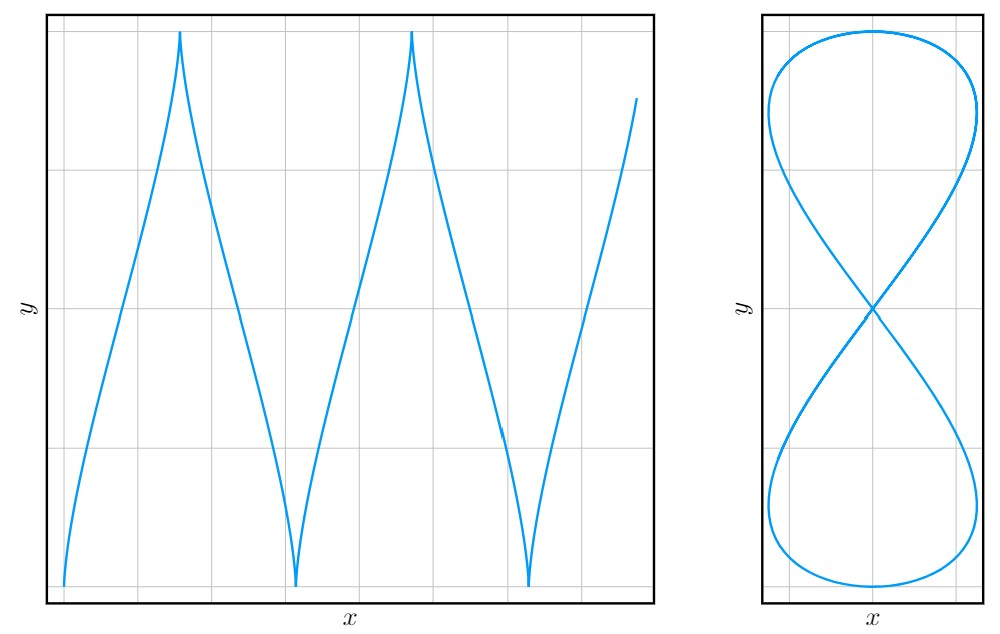
\includegraphics[width=.95\textwidth]{fig8}
	      \end{column}
	    \end{columns}
	\end{itemize}
\end{frame}

\subsection{The Ponderomotive force}

%%%%%%%%%%%%%%%%%%%%%%%%%%%% slide 5 %%%%%%%%%%%%%%%%%%%%%%%%%%%%

\begin{frame}{The Ponderomotive force}
  \begin{itemize}
	\item In a spatially uniform electric field an electron would oscillate around
  	its equilibrium position (in a figure 8 pattern).
  	\item If there is a spatial gradient of the field, a ponderomotive force will
  	appear
  	\[
  	F_p = -\frac{e^2}{4m \omega^2} \grad{\vb{E}}^2
  	\]
	\end{itemize}
\end{frame}

%%%%%%%%%%%%%%%%%%%%%%%%%%%% slide 6 %%%%%%%%%%%%%%%%%%%%%%%%%%%%

\begin{frame}{Laser Wakefield}
  \begin{itemize}
    \item When a high intensity laser propagates in plasma, the
	electric field pushes the electrons far away from their equilibrium
	position (via the ponderomotive force). This is known as the ``blowout phase''.
	\item This creates a high intensity field between the electrons and the
	nuclei left behind. Any charged particles trapped in this region will be accelerated.
	\item This low density bubble propagates through the plasma as the laser advances.
	\end{itemize}
\end{frame}

\section{The Particle in Cell Method}

\subsection{Particle Pusher}

\begin{frame}
	\begin{itemize}
		\item Solves the equations of motion for the electron
		\begin{subequations}
		  \begin{align*}
		    \frac{\vb{x}_{n+1}-\vb{x}_n}{\Delta t} &= \vb{v}_{n+1} \\
		    \frac{\vb{v}_{n+1/2}-\vb{v}_{n-1/2}}{\Delta t} &= \frac{q}{m}
		      \left(\vb{E}(\vb{x}_n) + \frac{\vb{v}_{n+1/2}+\vb{v}_{n-1/2}}{2} \cp \vb{B}(\vb{x}_n)\right)
		  \end{align*}
		\end{subequations}
		\item The Boris push algorithm: the motion is decomposed in the contribution from the electric
		and magnetic field.
	\end{itemize}
\end{frame}

\begin{frame}
	\begin{figure}
		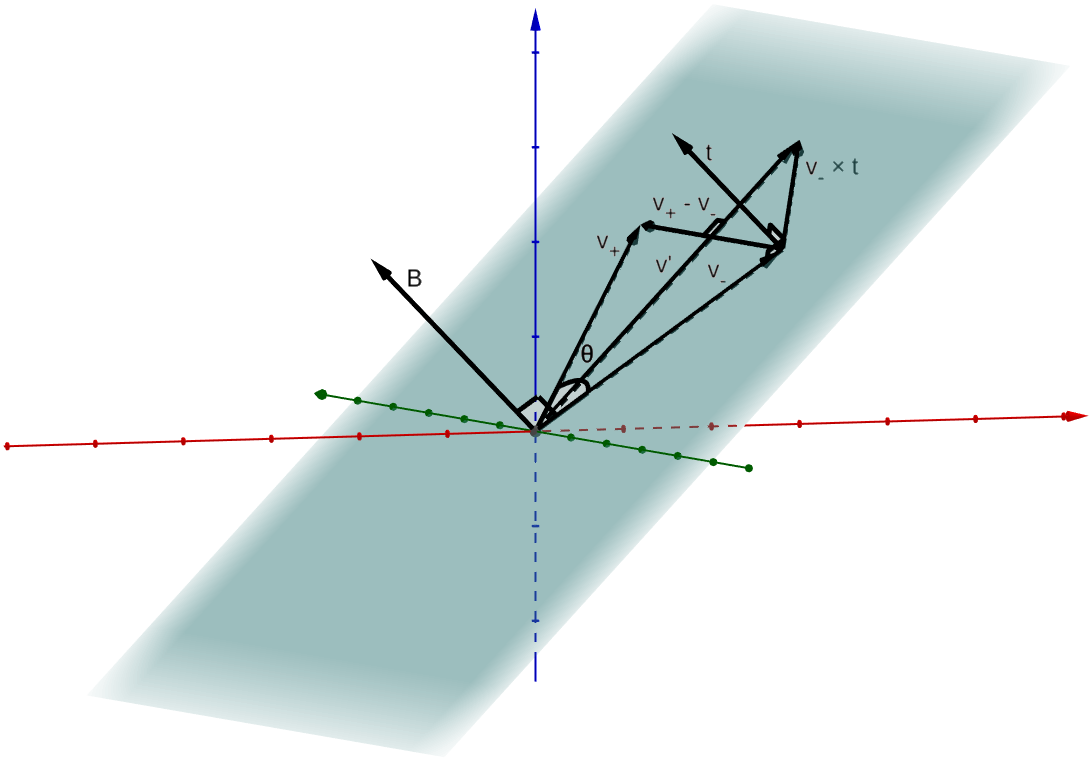
\includegraphics[width=\textwidth]{Boris-rotation-3D}
	\end{figure}
\end{frame}

\begin{frame}{The Boris push}
	\begin{enumerate}
	  \item \(\vb{v}^- = \vb{v}_{n-1/2} + \frac{q \vb{E}}{m} \frac{\Delta t}{2}\)
	  \item rotate \(\vb{v}^-\) to obtain \(\vb{v}^+\) using
	  \begin{enumerate}
	    \item \(\vb{v}' = \vb{v}^- + \vb{v}^- \cp \vb{t}\), where \(\vb{t} = \frac{q \vb{B}}{m} \frac{\Delta t}{2}\)
	    \item \(\vb{v}^+ = \vb{v}^- + \vb{v}' \cp \vb{s}\), where \(\vb{s} = \frac{2 \vb{t}}{1+t^2}\)
	  \end{enumerate}
	  \item \(\vb{v}_{n+1/2} = \vb{v}^+ + \frac{q \vb{E}}{m} \frac{\Delta t}{2}\)
	\end{enumerate}
\end{frame}

\begin{frame}{Conservation properties}
	\begin{itemize}
		\item We want the algorithm to be as close as possible to
		the original continuous system in terms of symmetries and conserved
		quantities.
		\item A linear map \(A: \mathbb{R}^{2d} \to \mathbb{R}^{2d}\) is called
  		\emph{symplectic} if
		  \[
		  A^T J^{-1} A = J^{-1},\qquad \text{where} \ J = \mqty(0 & I \\ -I & 0)\,,
		  \]
		\item The Boris push algorithm is not symplectic, but it is volume preserving.
	\end{itemize}
\end{frame}

\subsection{The Field solver}

\begin{frame}{The Field solver}
	\begin{itemize}
		\item Solve Maxwell's equations using
		\begin{align*}
		  \pdv{\vb{B}}{t} & = - \curl{\vb{E}} \\
		  \pdv{\vb{E}}{t} & = c^2 \curl{\vb{B}} - \frac{1}{\varepsilon_0} \vb{j}\,.
		\end{align*}
		\item Let us consider the 1D case first
		\begin{subequations}%
			\small
		\begin{align*}
		    &\frac{B_y^{n+1/2}(k+\frac{1}{2}) - B_y^{n-1/2}(k+\frac{1}{2})}{\Delta t} =
		    - \frac{E_x^n(k+1) - E_x^n(k)}{\Delta z} \\
		    &\frac{E_x^{n+1}(k) - E_x^{n}(k)}{\Delta t} =
		    -c^2 \frac{B_y^{n+1/2}(k+\frac{1}{2}) - B_y^{n+1/2}(k-\frac{1}{2})}{\Delta z}
		    -\frac{1}{\varepsilon_0} j_x^{n+1/2}(k) \,.
		\end{align*}
		\end{subequations}
	\end{itemize}
\end{frame}

\begin{frame}
	\begin{itemize}
		\begin{columns}[T, onlytextwidth]
	      \begin{column}{0.07\textwidth}

	      \end{column}
	      \begin{column}{0.3\textwidth}
		  \item Yee's method uses a leapfrog-like algorithm for staggering in both
		  space and time.
		  \item Continuity equations for \(\vb{E}\) and \(\vb{B}\) are
		  automatically satisfied at cell boundaries.
	      \end{column}
	      \begin{column}{0.7\textwidth}
		  	\vspace{15mm}
	        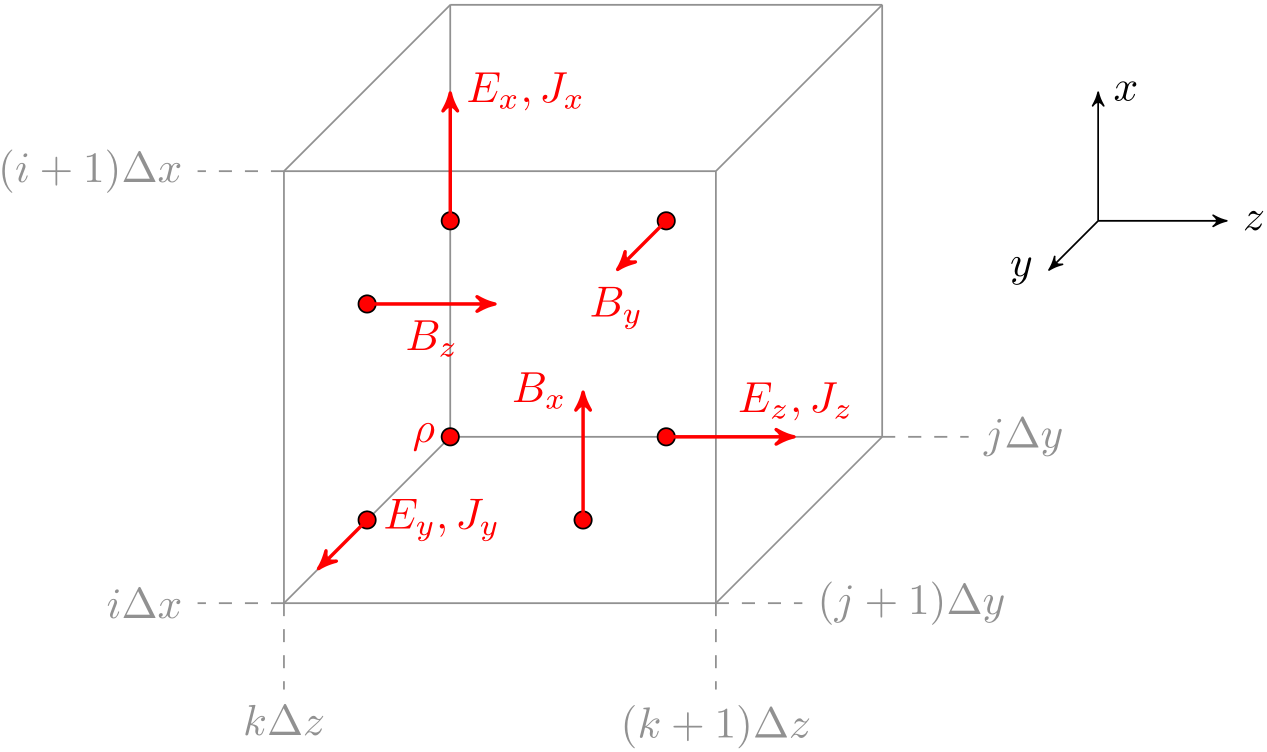
\includegraphics[width=.95\textwidth]{yee}
	      \end{column}
	    \end{columns}
	\end{itemize}
\end{frame}

\begin{frame}{The 3D case}
	\begin{itemize}
		\item The magnetic field is given by
		\[
		\mathcolor{green}{\pdv{B_y}{t}} = -\mathcolor{blue}{\pdv{E_x}{z}} + \mathcolor{magenta}{\pdv{E_z}{x}}
		\]
		\item which is discretized as
		\begin{equation*}
		\small
		  \begin{aligned}
		    &\frac{\mathcolor{green}{B_y^{n+1/2}}(\mathcolor{magenta}{i+\frac{1}{2}},j,\mathcolor{blue}{k+\frac{1}{2}})
		    - \mathcolor{green}{B_y^{n-1/2}}(\mathcolor{magenta}{i+\frac{1}{2}},j,\mathcolor{blue}{k+\frac{1}{2}})}{\mathcolor{green}{\Delta t}} = \\
		    &- \frac{\mathcolor{blue}{E_x}^{\mathcolor{green}{n}}(\mathcolor{magenta}{i+\frac{1}{2}},j,\mathcolor{blue}{k+1}) -
		      \mathcolor{blue}{E_x}^{\mathcolor{green}{n}}(\mathcolor{magenta}{i+\frac{1}{2}},j,\mathcolor{blue}{k})}{\mathcolor{blue}{\Delta z}}
		    \\&+ \frac{\mathcolor{magenta}{E_z}^{\mathcolor{green}{n}}(\mathcolor{magenta}{i+1},j,\mathcolor{blue}{k+\frac{1}{2}}) -
		      \mathcolor{magenta}{E_z}^{\mathcolor{green}{n}}(\mathcolor{magenta}{i},j,\mathcolor{blue}{k+\frac{1}{2}})}{\mathcolor{magenta}{\Delta x}}
		  \end{aligned}
		\end{equation*}
		\item or
		\[
		\partial_t B_y \rvert^n_{i+\frac{1}{2},j,k+\frac{1}{2}} =
		  -\partial_z E_x \rvert^n_{i+\frac{1}{2},j,k+\frac{1}{2}}
		  +\partial_x E_z \rvert^n_{i+\frac{1}{2},j,k+\frac{1}{2}}
		\]
	\end{itemize}
\end{frame}

\begin{frame}{What about the other equations?}
	\begin{itemize}
		\item For \(\div{\vb{B}} = 0 \)
		\[
		\pdv{\div{\vb{B}}}{t} = \div{\pdv{\vb{B}}{t}} = \div{\left(-\curl{\vb{E}}\right)} = 0\,.
		\]
		\item For \(\div{\vb{E}} = \frac{\rho}{\varepsilon_0}\)
		\[
		\begin{aligned}
			\pdv{t} \left(\div{\vb{E}} - \frac{\rho}{\varepsilon_0}\right) &=
			-\frac{1}{\varepsilon_0} \left[\pdv{\rho}{t}
			-\div{\left(\frac{1}{\mu_0} \curl{\vb{B}} - \vb{j}\right)}\right]\\ &=
			-\frac{1}{\varepsilon_0} \left(\pdv{\rho}{t} + \div{\vb{j}}\right)
		\end{aligned}
		\]
	\end{itemize}
\end{frame}

%%%%%%%%%%%%%%%%%%%%%%%%%%%% slide 8 %%%%%%%%%%%%%%%%%%%%%%%%%%%%

\begin{frame}{Numerical Stability}
  \begin{itemize}
    \item In order to accurately represent the physics, the temporal
		and spatial discretizations must be chosen appropriately.
		\item For the spatial discretizations, the dimension of a cell must be
		significantly smaller than the laser wavelength.
		\[
		D_{cell} \ll \lambda_L
		\]
		\item The timestep is then computed from the spatial discretizations
		automatically via the Courant condition.
		\[
		c \Delta t \leq \frac{1}{\sqrt{\frac{1}{\Delta x^2} + \frac{1}{\Delta y^2} + \frac{1}{\Delta z^2}}}
		\]
  \end{itemize}
\end{frame}


\subsection{PIC in practice}

\begin{frame}
	\begin{itemize}
		\item PIC codes require significant computational resources (HPC).
		\item The implementation must take advantage of all the available
		computing resources (MIP, SIMD, CUDA).
		\item Scalability is crucial for employing large parallel simulations.
		\item Amdahl's law
		\[
		S_A = \frac{1}{(1-p)+\frac{p}{n}}
		\qquad \text{and} \qquad
		\lim_{n\to\infty} S_A = \frac{1}{1-p}
		\]
	\end{itemize}
\end{frame}

%%%%%%%%%%%%%%%%%%%%%%%%%%%% slide 10 %%%%%%%%%%%%%%%%%%%%%%%%%%%%

\begin{frame}
	\begin{figure}
		\includestandalone[width=\textwidth]{../figures/theoretical-scaling-Amdahl}%
		\caption{The speedup computed with Amdahl's law}
	\end{figure}
\end{frame}

% %%%%%%%%%%%%%%%%%%%%%%%%%%%% slide 11 %%%%%%%%%%%%%%%%%%%%%%%%%%%%
%
\begin{frame}
	\begin{figure}
		\includestandalone[width=\textwidth]{../figures/theoretical-scaling-all}%
		\caption{The theoretical speedup compared with linear axis and small number
	  of processors on the left and log-log scale with a large number of processors
	  on the right}
	\end{figure}
\end{frame}

\section{Results}

% %%%%%%%%%%%%%%%%%%%%%%%%%%%% slide 13 %%%%%%%%%%%%%%%%%%%%%%%%%%%%
%
\begin{frame}{Solid targets}
	\begin{figure}[h]
	  \centering
	  \begin{subfigure}[b]{0.475\textwidth}
	    \centering
	    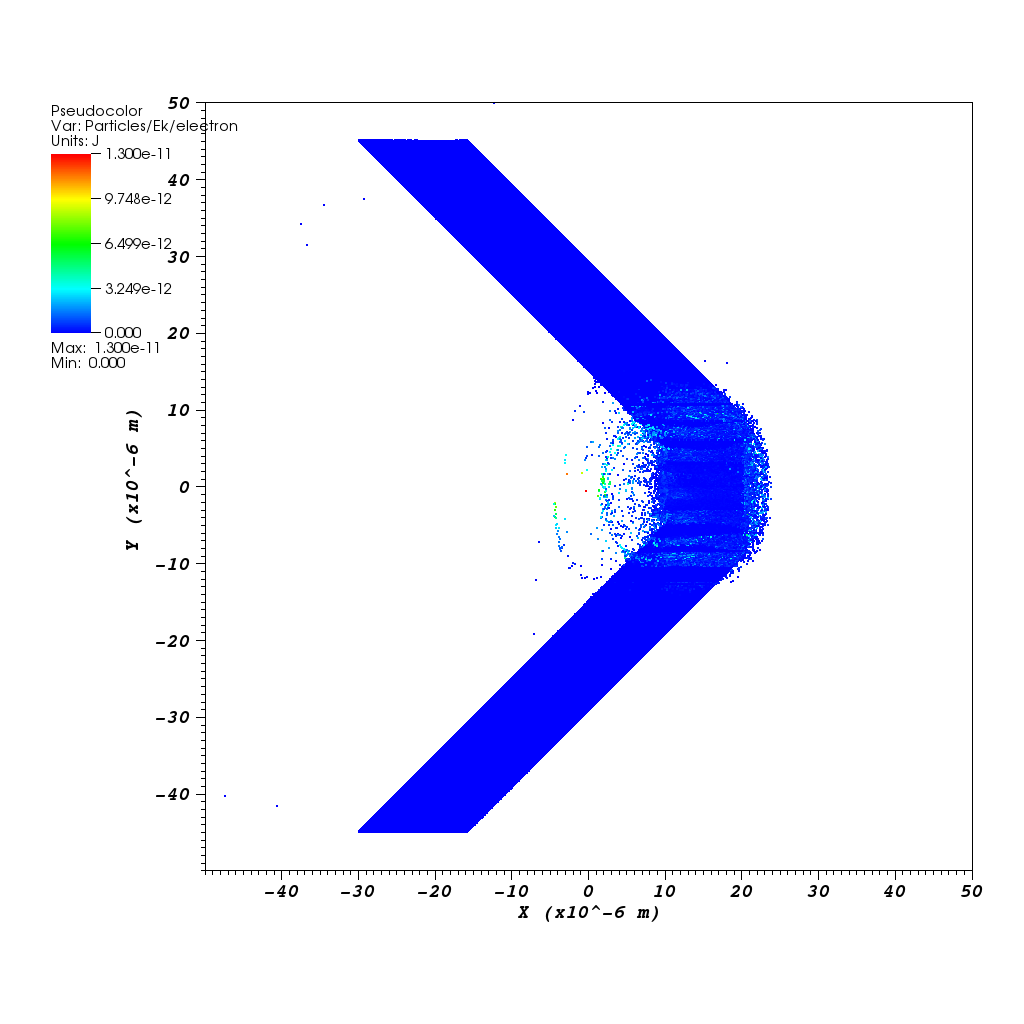
\includegraphics[width=\textwidth]{i21-ek-init-e}
	    \caption{The kinetic energy of the electrons right after the pulse
	    hits the cone}%
	  \end{subfigure}
	  \hfill
	  \begin{subfigure}[b]{0.475\textwidth}
	    \centering
	    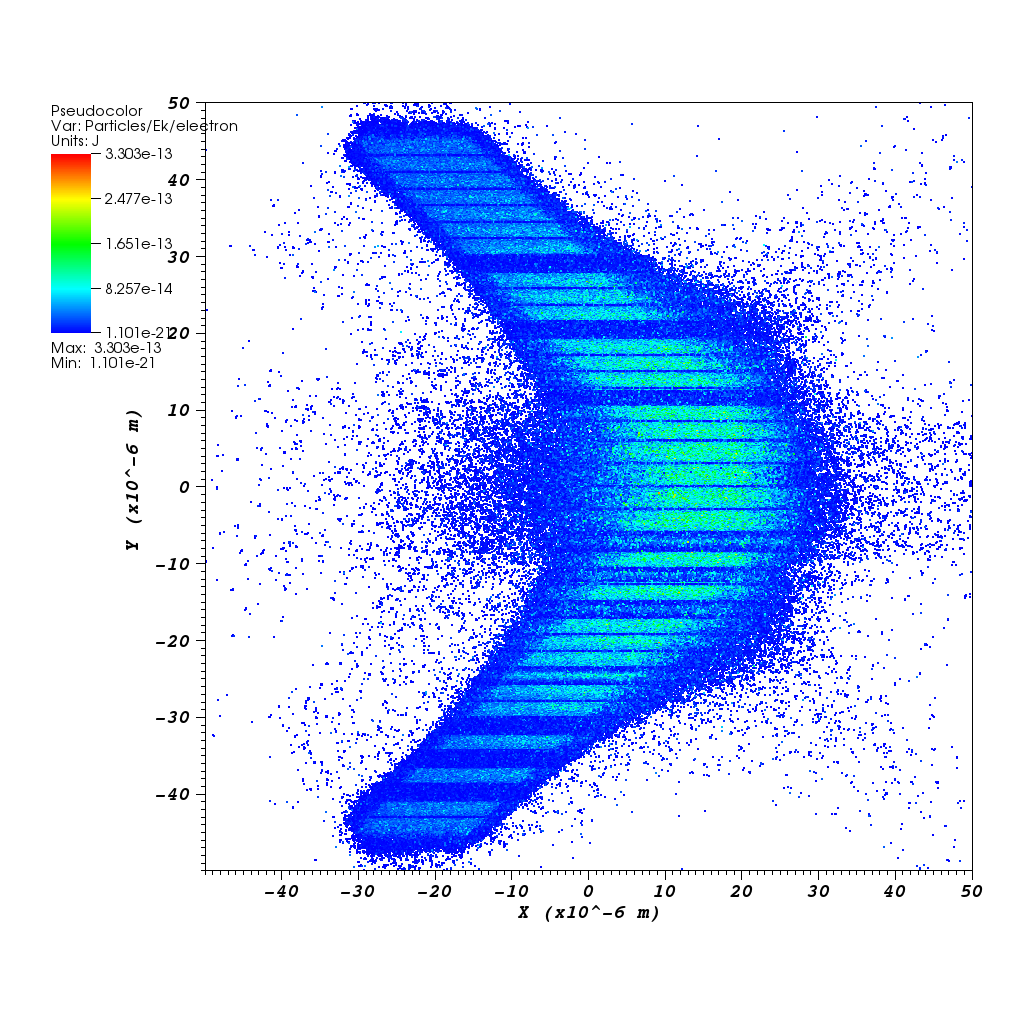
\includegraphics[width=\textwidth]{i21-ek-end-e}
	    \caption{The kinetic energy of the electrons a long time after the pulse
	    hits the cone}%
	  \end{subfigure}
	  \caption{The kinetic energy of the electrons for the
	  \(I=\SI{e21}{\watt\per\centi\metre\squared}\) laser pulse}%
	\end{figure}
\end{frame}

\begin{frame}
	\begin{figure}[h]
	  \centering
	  \begin{subfigure}[b]{0.475\textwidth}
	    \centering
	    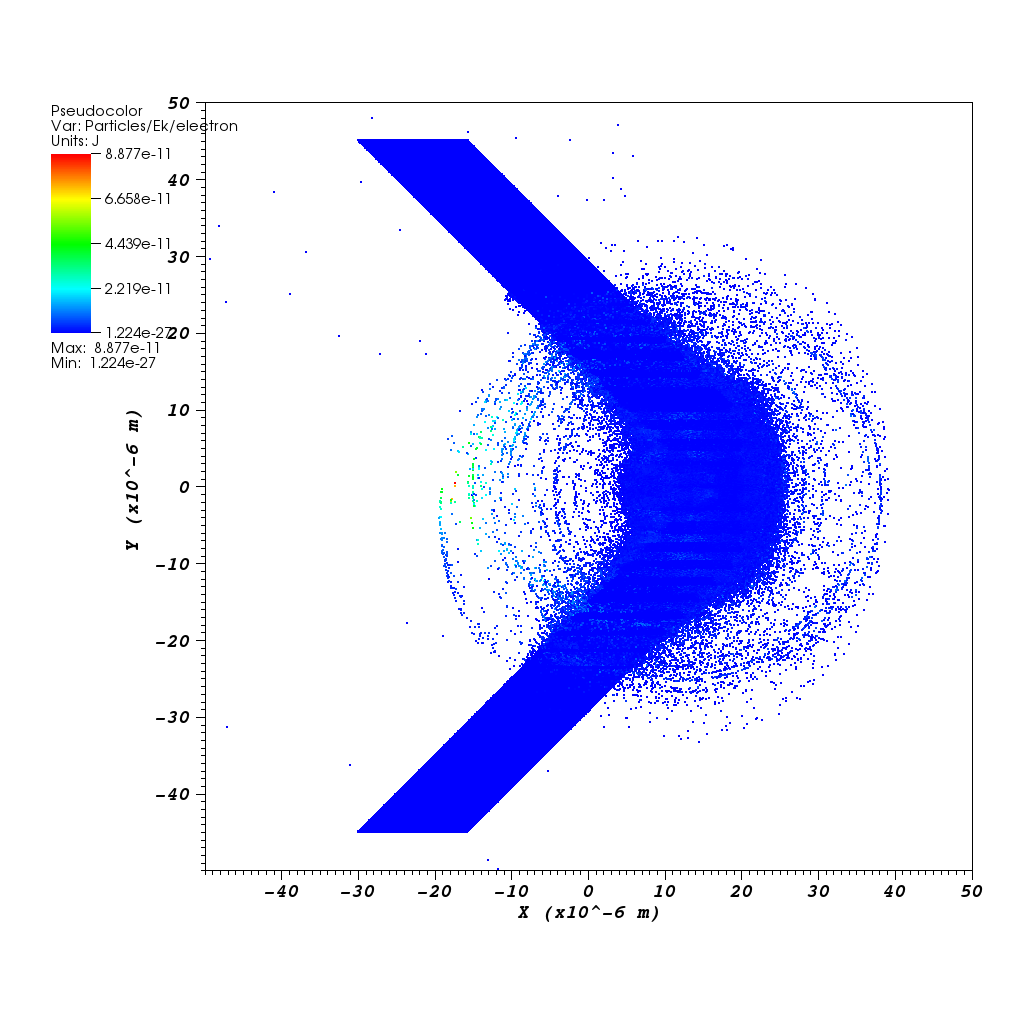
\includegraphics[width=\textwidth]{i22-ek-init-e}
	    % \caption{The kinetic energy of the electrons right after the pulse
	    % hits the cone}%
	  \end{subfigure}
	  \hfill
	  \begin{subfigure}[b]{0.475\textwidth}
	    \centering
	    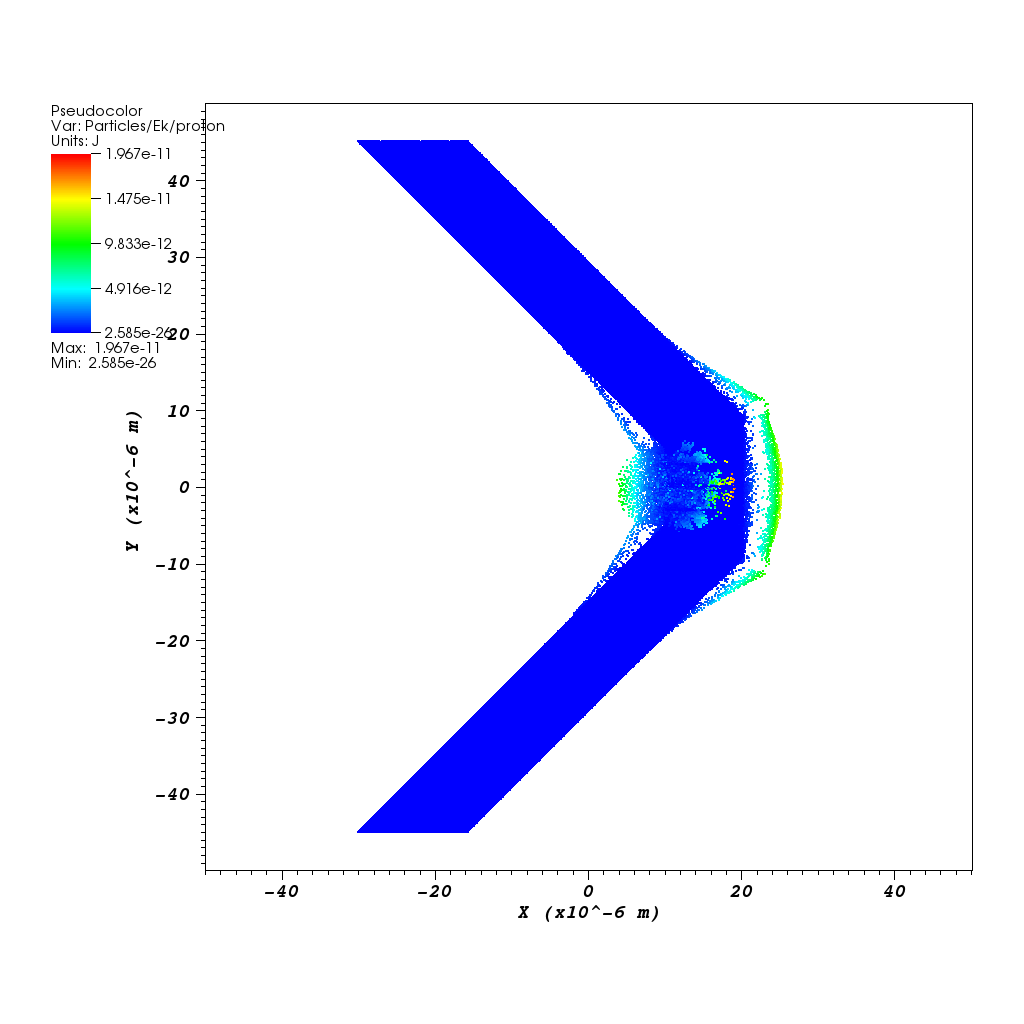
\includegraphics[width=\textwidth]{i22-ek-init-p}
	    % \caption{The kinetic energy of the protons right after the pulse
	    % hits the cone}%
	  \end{subfigure}
	  \caption{The kinetic energy of the electrons and protons for the
	  \(I=\SI{e22}{\watt\per\centi\metre\squared}\) laser pulse}%
	\end{figure}
\end{frame}

% %%%%%%%%%%%%%%%%%%%%%%%%%%%% slide 19 %%%%%%%%%%%%%%%%%%%%%%%%%%%%
%
\begin{frame}{Gaseous targets}
	\begin{figure}
		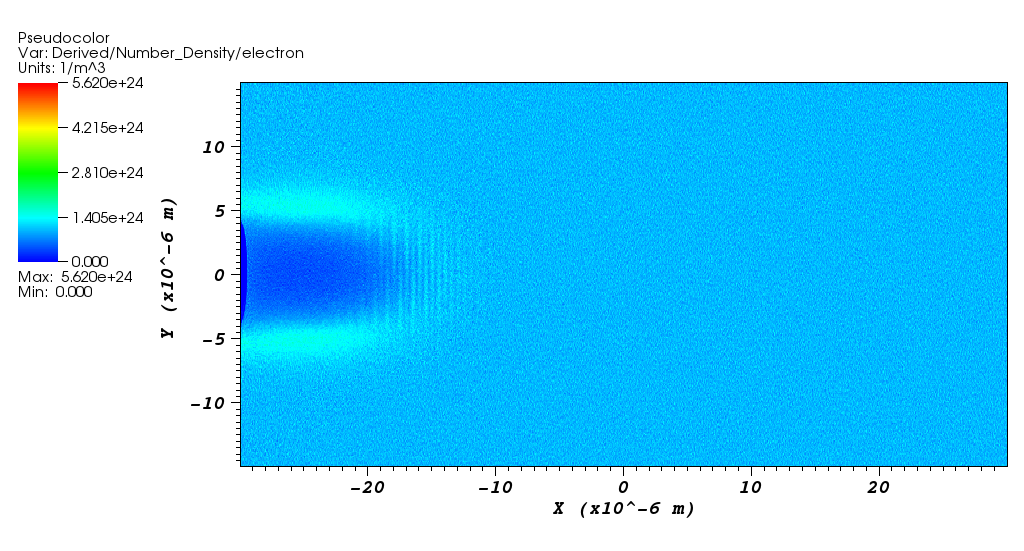
\includegraphics[width=\textwidth]{lwfa-i18-n-init-e}
	\end{figure}
\end{frame}

\begin{frame}
	\begin{figure}
		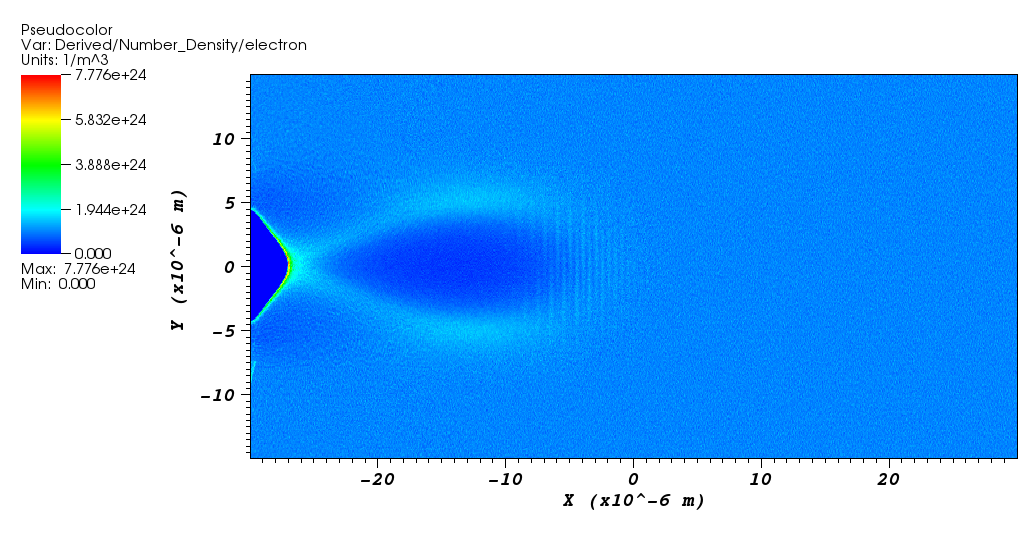
\includegraphics[width=\textwidth]{lwfa-i18-n-init1-e}
	\end{figure}
\end{frame}

\begin{frame}
	\begin{figure}
		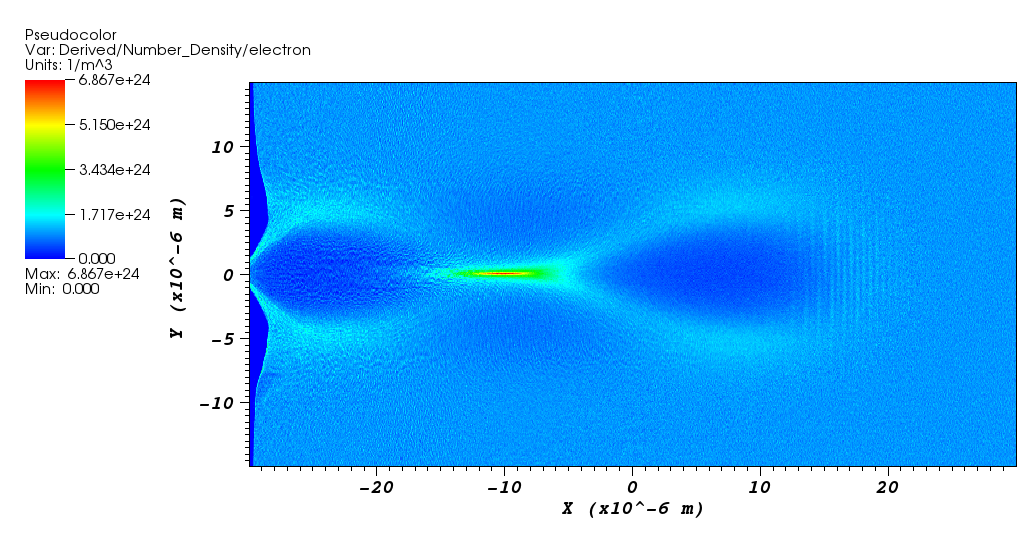
\includegraphics[width=\textwidth]{lwfa-i18-n-mid-e}
	\end{figure}
\end{frame}

\begin{frame}
	\begin{figure}
		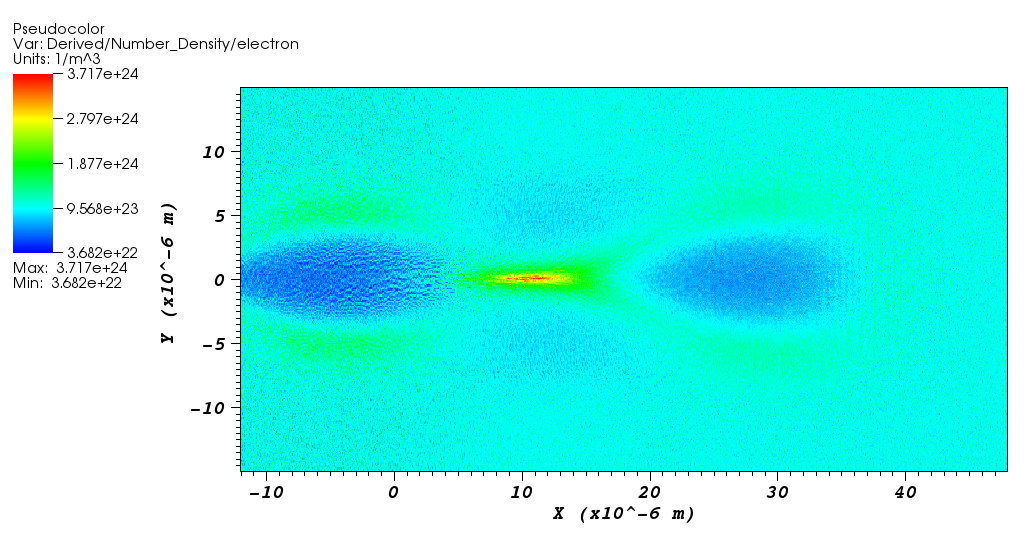
\includegraphics[width=\textwidth]{lwfa-i18-n-mid1-e}
	\end{figure}
\end{frame}


\begin{frame}
	\begin{figure}[h]
	  \centering
	  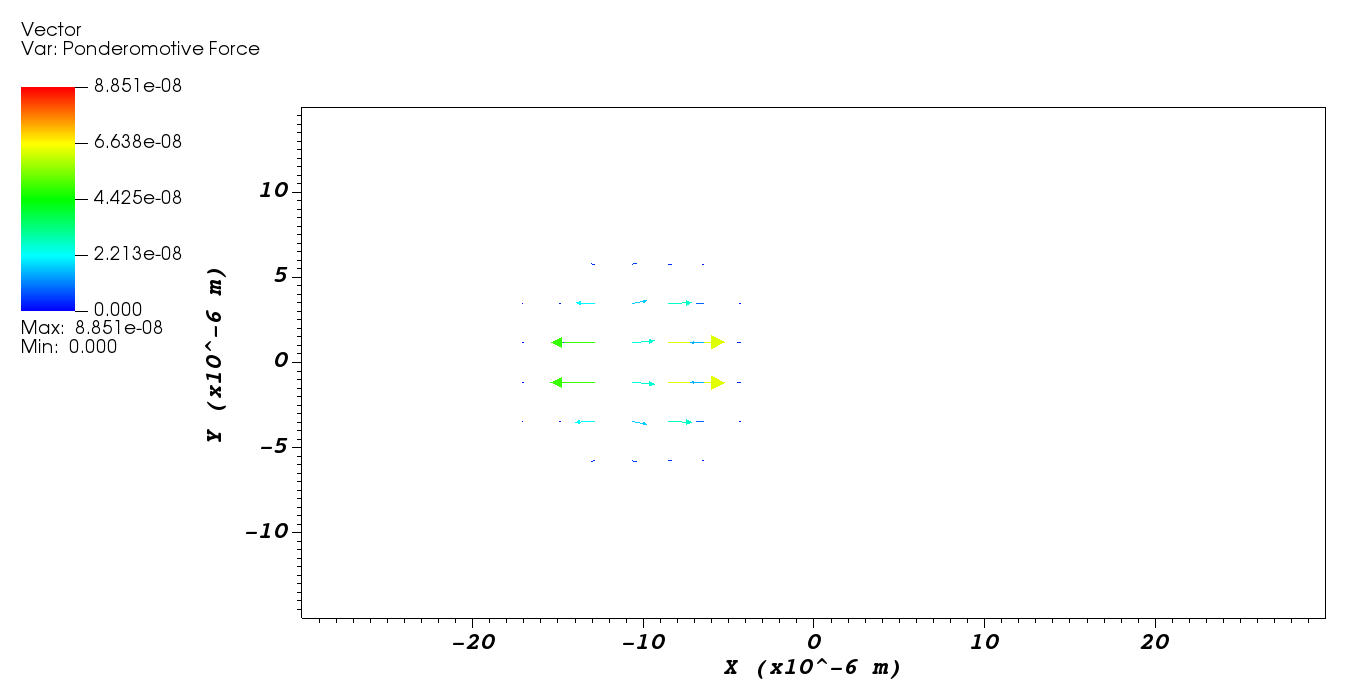
\includegraphics[width=\textwidth,height=0.5\textheight]{lwfa-i18-pond-f}
	  \caption{The ponderomotive force for the \(I=\SI{e18}{\watt\per\centi\metre\squared}\)
	  laser pulse}%
	\end{figure}
\end{frame}

%%%%%%%%%%%%%%%%%%%%%%%%%%%% slide 32 %%%%%%%%%%%%%%%%%%%%%%%%%%%%

\section{Conclusions}

\begin{frame}{Conclusions}
	\begin{itemize}
		\item This thesis addresses the large field of laser plasma interactions in a
		computational framework.
		\item This thesis is devoted to a class of self-consistent methods of
		solving the dynamics of electrically charged particles in strong electromagnetic
		fields.
		\item The most prominent effect observed in my numerical simulations is the
		laser wakefield acceleration visible in the case of gaseous targets subjected
		to highly intense laser pulses.
	\end{itemize}
\end{frame}

%%%%%%%%%%%%%%%%%%%%%%%%%%%% slide 27 %%%%%%%%%%%%%%%%%%%%%%%%%%%%

\begin{frame}[standout]
Thank you!
\end{frame}

\end{document}
